\chapter{Theoretical background}

\section{Convolution Neural Network - CNN}

Convolutional neural network is a type of neural network\cite{masood2018real}. It is composed of neurons with learnable weights and biases. Each neuron receives input, performs a dot product, and optionally follows with a non-linear response. Convolution Layers, Pooling Layers, Activation Layers, and Fully Connected Layers are the main components of CNN. ConvNet architectures explicitly assume that the inputs are images, allowing us to encode specific properties into the architecture. This makes the forward function easier to implement and reduces the number of parameters in the network significantly. Image classification, object detection, semantic segmentation, face recognition, and so on are some of the primary applications of CNN.

%Insert picture about CNN https://scholarworks.iupui.edu/bitstream/handle/1805/24768/FINAL%20Prasham_Shah_Thesis%20.pdf?sequence=1&isAllowed=y
\begin{figure}[H]
	\centering
	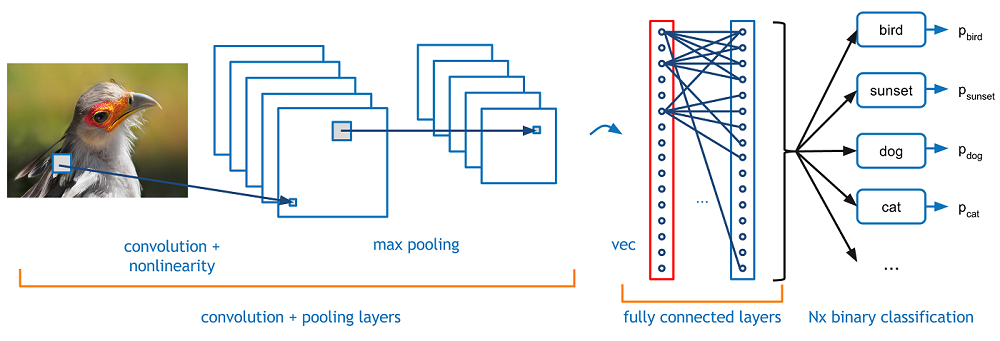
\includegraphics[width=\textwidth]{img/Chap3/Cover.png}
	\caption{Convolution Neural Network}
	\label{fig:Chap3-OverviewTheCNN}
\end{figure}

The Figure \ref{fig:Chap3-OverviewTheCNN} above shows an example of a convolution neural network, which is taking an image as input and then extracting features from it through various layers and then finally predicting the class of the object in the given image.

\subsection{Architecture}

Convolution Neural Networks have a different architecture with regular Neural Networks, and we can see this difference in Figure \ref{fig:Chap3-DiffArchCNN_NNN} below. Regular Neural Networks transform an input through a series of hidden layers. Every layer comprises a set of neurons, where each layer is fully connected to all neurons in the previous layers. Finally, a last fully-connected output layer represents the predictions with CNN architecture. First of all, the layers are organized into three dimensions: width, height, and depth. Further, the neurons in one layer do not connect to all neurons in the next layer but only to a small region. Lastly, the system will reduce the final output to a single vector of probability scores, organized along the depth dimension.

%FIXME: Insert image of diff architecture : https://www.freecodecamp.org/news/an-intuitive-guide-to-convolutional-neural-networks-260c2de0a050/
\begin{figure}[H]
	\centering
	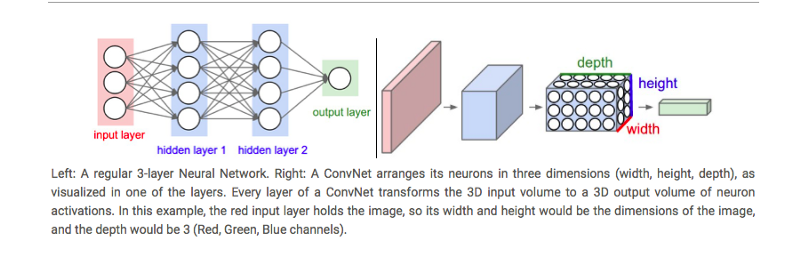
\includegraphics[width=\textwidth]{img/Chap3/DiffArchCNN-ANN}
	\caption{Different between Normal Neural Network and Convolution Neural Network}
	\label{fig:Chap3-DiffArchCNN_NNN}
\end{figure}

%FIXME: Insert image of CNN arc: https://www.freecodecamp.org/news/an-intuitive-guide-to-convolutional-neural-networks-260c2de0a050/
\begin{figure}[H]
	\centering
	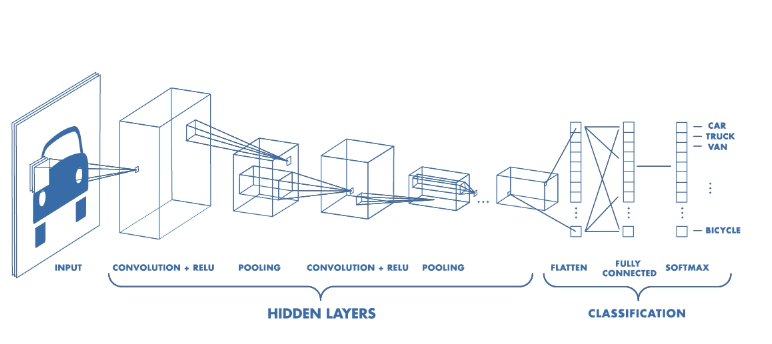
\includegraphics[width=\textwidth]{img/Chap3/CNN-Arch}
	\caption{Convolution Neural Network Architecture}
	\label{fig:Chap3-CNN_Arch}
\end{figure}

As we can see in Figure \ref{fig:Chap3-CNN_Arch}, CNN can be divided into two parts:
\begin{enumerate}
	\item The hidden layers/ Feature extraction part\\
	In this part, the network will perform a series of convolutions and pooling operations while the features are detected. Imagine you have a picture of a zebra, these are the parts where the
	network would recognize: its stripes, two ears, and four legs.
	\item The Classification part\\
	The fully connected layers serve as a classifier on top of their extracted features. By using a provided algorithm, they will assign a probability for the objects on the image.
\end{enumerate}

\subsection{Feature extraction part}
\subsubsection{Convolutional Layer}

The convolution layer is the core building block of a Convolutional Network that does most of the computational heavy lifting. A convolution is executed by sliding the filter over the input. At every location, matrix multiplication is performed and it sums the result onto the feature map. This extracting features from images happen throughout the CNN's convolutional layers. This process is illustrated in Figure \ref{fig:Chap3-CNN_Layer}

% FIXME: https://scholarworks.iupui.edu/bitstream/handle/1805/24768/FINAL%20Prasham_Shah_Thesis%20.pdf?sequence=1&isAllowed=y
\begin{figure}[H]
	\centering
	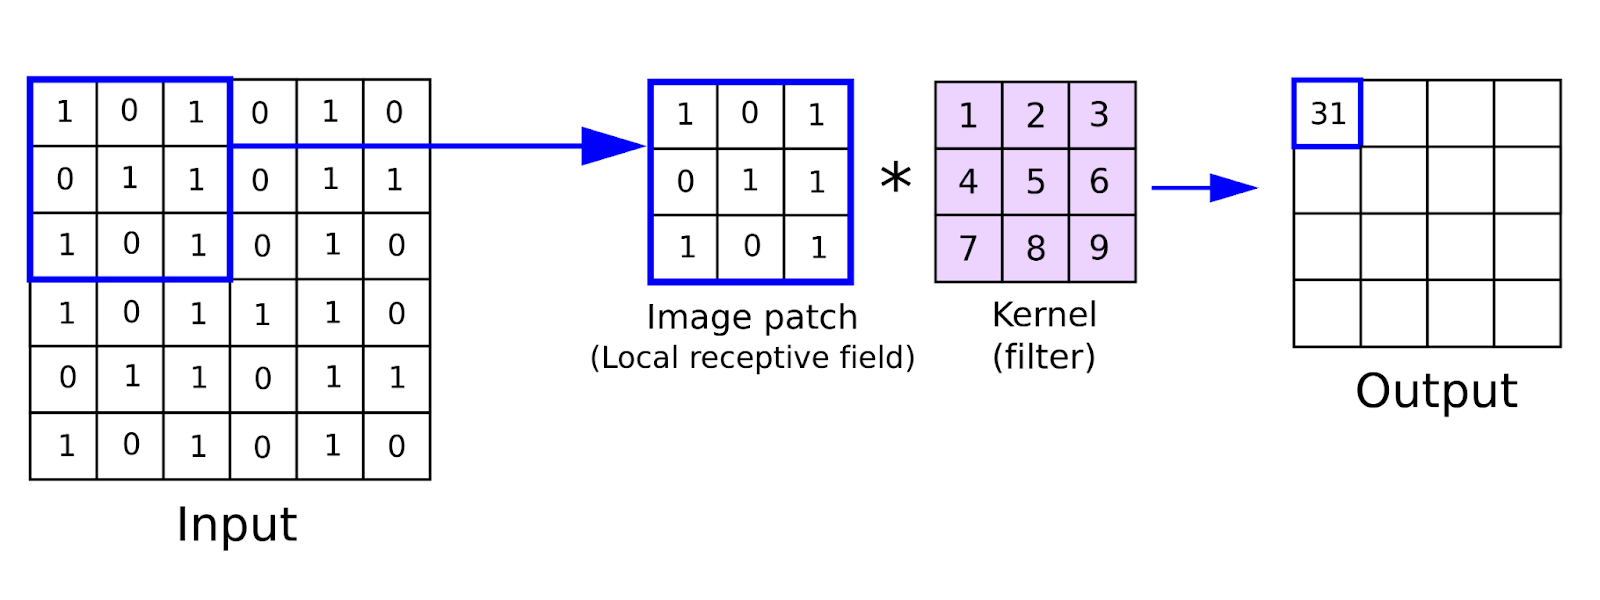
\includegraphics[width=\textwidth]{img/Chap3/ConvLayer}
	\caption{Convolution Neural Network Layer}
	\label{fig:Chap3-CNN_Layer}
\end{figure}

When the feature map is made, we can pass each value in the feature map through a non-linearity function, such as ReLU, sigmoid before it becomes the input of the next convolution layer.

Because the size of the feature map is always smaller than the input, we have to do something to prevent our feature map from shrinking. This is where we use padding (\ref{fig:Chap3-CNN_Padding}). A layer of zero-value pixels is added to surround the input with zeros so that our feature map will not shrink. In addition to keeping the spatial size constant after performing convolution, padding also improves performance, ensures the Kernel and strides size will fit in the input.

% FIXME: => Need picture
\begin{figure}[H]
	\centering
	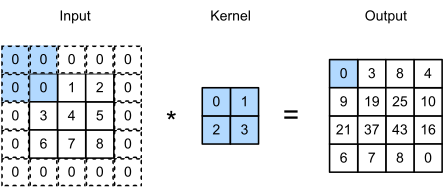
\includegraphics[width=\textwidth]{img/Chap3/CNN_Padding}
	\caption{Using padding for strike one in Convolution Layer}
	\label{fig:Chap3-CNN_Padding}
\end{figure}
\subsubsection{Pooling Layers}

After a convolution layer, it is common to add a pooling layer in between CNN layers. The function of Pooling is to continuously reduce the dimensionality to reduce the number of parameters and computation in the network. This action shortens the training time and controls overfitting.

There are two main types of Pooling Layers in a CNN: Max Pooling and Average Pooling. The functionality of these two types of layers is demonstrated in Figure \ref{fig:Chap3-CNN_Pooling}. Max Pooling restores the maximum value from the picture segment covered by the Kernel. Average Pooling converts the average values from the bit of the picture surrounded by the Kernel.

\begin{figure}[H]
	\centering
	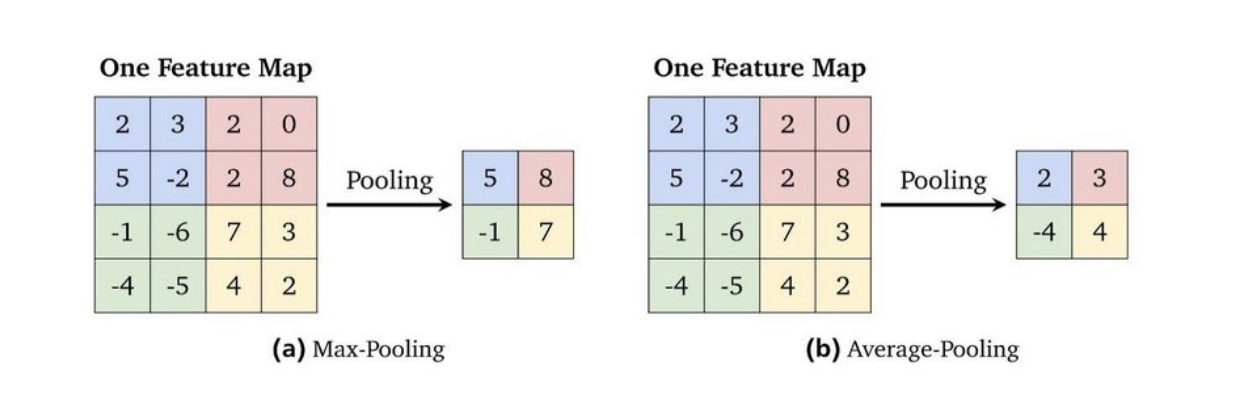
\includegraphics[width=\textwidth]{img/Chap3/Pooling}
	\caption{Max Pooling and Average Pooling}
	\label{fig:Chap3-CNN_Pooling}
\end{figure}

% FIXME: Insert image about max pooling and average pooling

\subsubsection{Activation Layers}

In general, Neural networks and CNNs rely on a non-linear "trigger" function to signal distinct identification of likely features on each hidden layer. CNN may use a variety of specific functions (Figure \ref{fig:Chap3-CNN_ActiveFunction}), such as rectified linear units (ReLUs) and continuous trigger (non-linear) functions—to efficiently implement this non-linear triggering.

\begin{figure}[H]
	\centering
	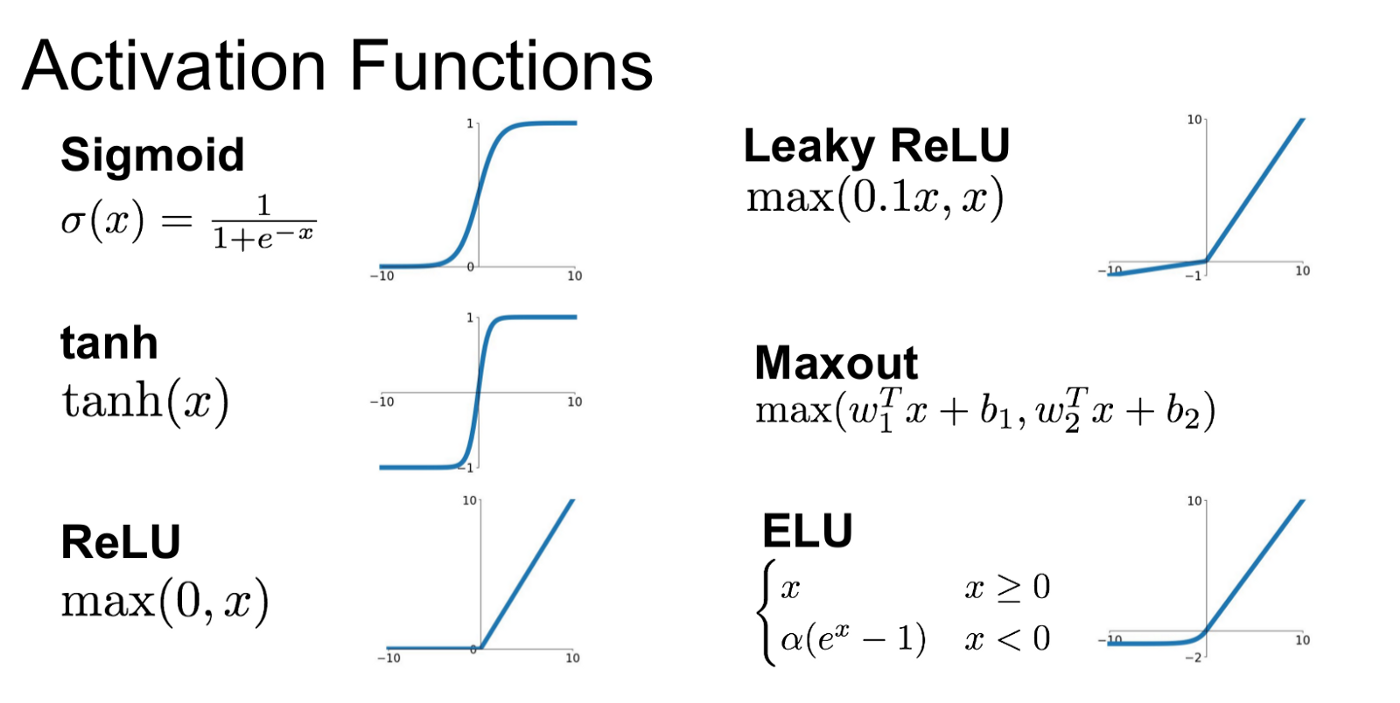
\includegraphics[width=\textwidth]{img/Chap3/ActiveFunction}
	\caption{ Some Active Function common used in CNN }
	\label{fig:Chap3-CNN_ActiveFunction}
\end{figure}
% FIXME: Insert picture of some function like ReLU, tanh ....
\subsection{Classification part}
\subsubsection{Fully connected layers}

The last layers of a CNN are fully connected. Neurons in a fully connected layer have complete connections to all the activations in the previous layer. This part is, in principle, the same as a regular Neural Network.

Figure \ref{fig:Chap3-FC} illustrates the way of input value stream into the fully connected layer. Because these fully connected layers can only accept one-dimensional data, we need to convert our 3D data to 1D data. After passing through some FC, we will get the data classification result.

\begin{figure}[H]
	\centering
	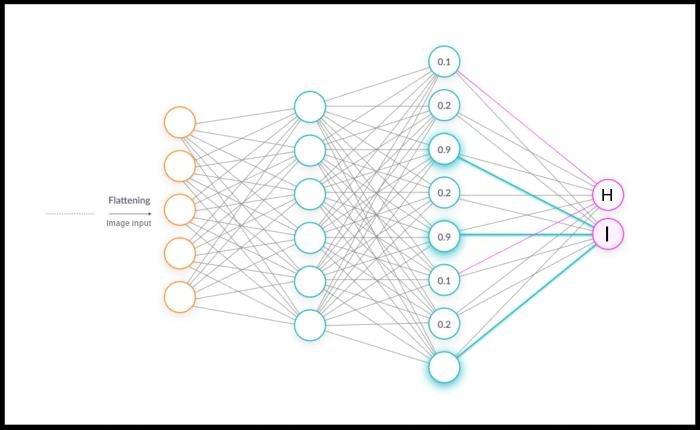
\includegraphics[width=\textwidth]{img/Chap3/FC}
	\caption{ Fully connected layer}
	\label{fig:Chap3-FC}
\end{figure}
% FIXME: Insert picture ...
\section{Media Pipe}\label{sec:MediaPipe}
% FIXME: Lấy từ eureka bỏ vào
\subsection{Introduction to Media Pipe Hands}
MediaPipe Hands (\ref{fig:Chap3-MediaPipe}) is a high-resolution tracking system for hands and fingers\cite{zhang2020mediapipe}. It uses machine learning to infer 21 3D hand landmarks from a single frame. This solution delivers real-time performance on a cell phone and even scales to many hands, whereas current state-of-the-art systems rely primarily on powerful desktop environments for inference.

\begin{figure}[H]
	\centering
	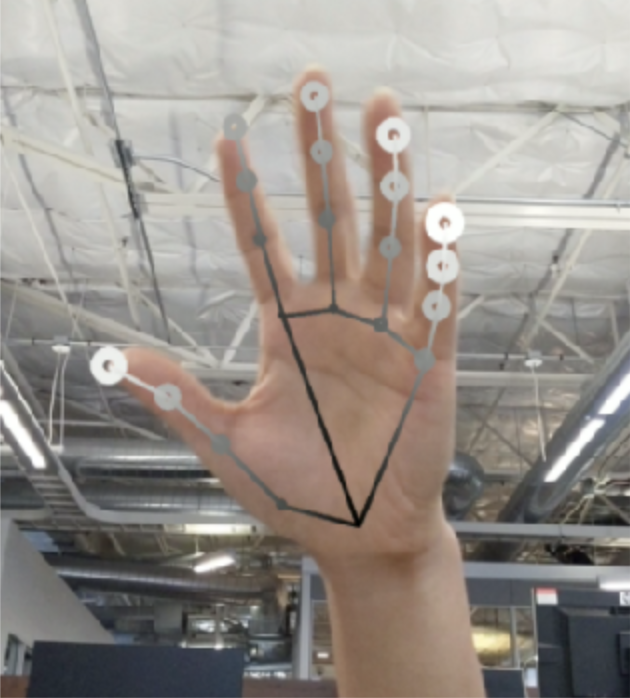
\includegraphics[width=0.8\textwidth]{img/Chap3/Media Pipe}
	\caption{ Media Pipe real time tracking 3D hand landmarks}
	\label{fig:Chap3-MediaPipe}
\end{figure}

MediaPipe Hands makes use of a machine learning pipeline that consists of several models that work together: A palm detection model, which acts on the entire image, will return an orientated hand bounding box. A hand landmark model that returns high-fidelity 3D hand key points from the cropped image region determined by the palm detector.

However, providing the hand landmark model with a correctly cropped hand image minimizes the requirement for data augmentation drastically (such as rotations, translations, and scaling) and instead, allows the network to focus on coordinate prediction accuracy. Furthermore, in this ML pipeline, crops can be created based on the hand landmarks recognized in the previous frame, and palm detection is only used to localize the hand when the landmark model can no longer detect its presence.
\subsection{Palm detection model}
The Media Pipe team provides the palm detection model to detect initial hand locations and distinguish whether the hand recognized is left or right, which is very useful as each sign goes along with a different side will result in different meanings. They created a single-shot detector model, comparable to the face detection model in MediaPipe Face Mesh\cite{MediaPipeFaceMesh}, tailored for mobile real-time applications. Hand detection is difficult: our model must detect occluded and self-occluded hands and work across many hand sizes with a significant scale span relative to the image frame.

According to their statements, the methods they used to address the above challenges vary in many strategies. First, instead of training a hand detector, they trained a palm detector because estimating bounding boxes of inflexible objects like palms and fists was much easier than recognizing hands with articulated fingers. Furthermore, the non-maximum suppression method performs effectively even in two-hand self-occlusion situations such as handshakes because palms are small objects. Furthermore, palms can be simulated using square bounding boxes (anchors in ML language) that ignore other aspect ratios, reducing 3-5 anchors. Second, even for tiny objects, an encoder-decoder feature extractor is used for more extensive picture context awareness (similar to the Retina Net approach). Finally, the significant scale variance limits focus loss during training to support many anchors.

Using the strategies described above gives an average precision of 95.7 percent in palm detection. With no decoder and a regular cross-entropy loss, the baseline is just 86.22 percent.

\subsection{Hand landmark model}
Following palm detection over the entire image, our next hand landmark model uses regression to accomplish exact key point localization of 21 3D hand-knuckle coordinates (see Figure \ref{fig:Chap3-HandLandMark}) within the detected hand regions, i.e., direct, coordinate prediction. Even with partially visible hands and self-occlusions, the model develops a consistent internal hand posture representation.
\begin{figure}[H]
	\centering
	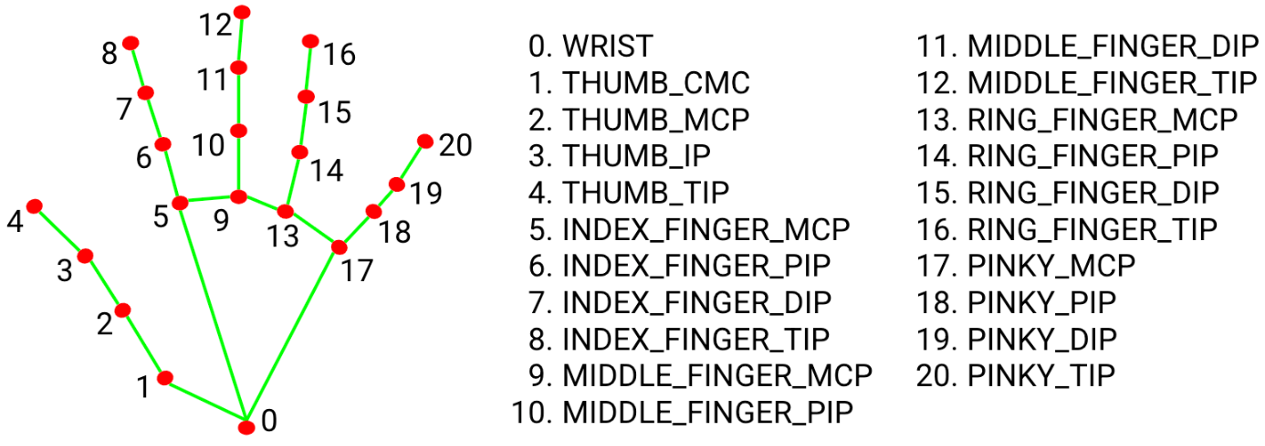
\includegraphics[width=\textwidth]{img/Chap3/HandLandMark}
	\caption{ 21 hand landmarks }
	\label{fig:Chap3-HandLandMark}
\end{figure}


\section{Distance matrix}

A distance matrix\cite{DistanceMatrix} is a table that shows the distance between pairs of objects. For example, in the Figure \ref{fig:Chap3-DM}., we can see the length between A and B is 16, B and C is 37, and so on. The diagonal of the table is the distance to the object from itself, so the value, as we can see, is 0. Distance matrices are sometimes called dissimilarity matrices.

\begin{figure}[H]
	\centering
	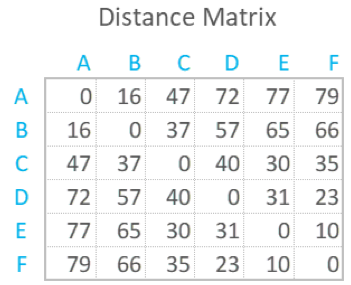
\includegraphics[width=0.6\textwidth]{img/Chap3/DM}
	\caption{ Distance matrix }
	\label{fig:Chap3-DM}
\end{figure}

% FIXME: Insert picture of distance matrix

\subsection{Create distance matrix}

A distance matrix is computed from a raw data table. In the example below (Figure \ref{fig:Chap3-DM_Formula}), we can use high school math (Pythagoras) to work out the distance between A and B.

% FIXME: Chèn công thức vào đây
\begin{figure}[H]
	\centering
	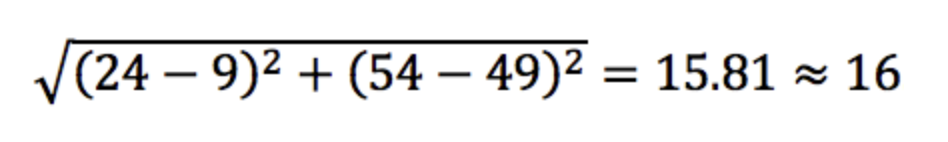
\includegraphics[width=0.7\textwidth]{img/Chap3/DM_Formula}
	\caption{ Calculating distance between A and B}
	\label{fig:Chap3-DM_Formula}
\end{figure}

We can use the same formula with more than two variables, known as the Euclidean distance. As a result, we have the distance matrix represented like Figure \ref{fig:Chap3-DM-Raw}.

% FIXME: chèn bảng kết quả vào
\begin{figure}[H]
	\centering
	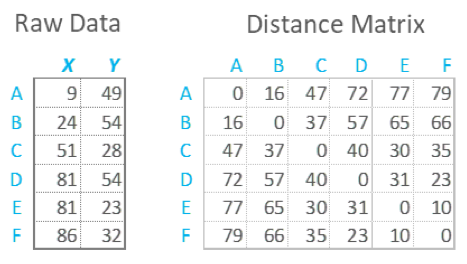
\includegraphics[width=0.7\textwidth]{img/Chap3/DM-Raw}
	\caption{ The distance matrix is constructed from raw data }
	\label{fig:Chap3-DM-Raw}
\end{figure}

\section{Beam search and Connectionist Temporal Classification}
% CheckList:
%   [x] BeamSearch
%   [x] CTC recap
%   [x] Combination
%   [x] Pseudo code
\subsection{Connectionist Temporal Classification}

Connectionist Temporal Classification (CTC)\cite{hannun2017sequence} is a type of Neural Network output helpful in tackling sequence problems like handwriting (Figure \ref{fig:Chap3-Overview-CTC}) and speech recognition where the timing varies. Using CTC ensures that one does not need an aligned dataset, which makes the training process
more straightforward.

% FIXME: Insert about CTC in speech recognition
\begin{figure}[H]
	\centering
	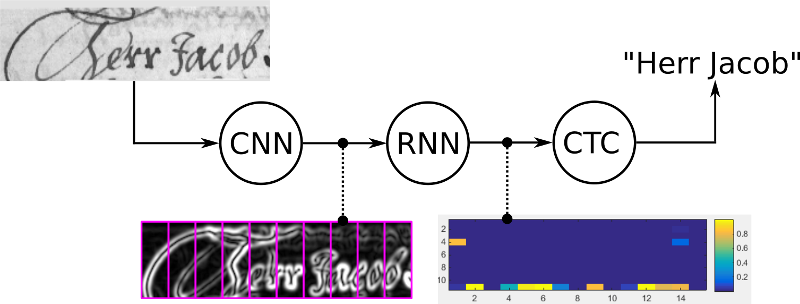
\includegraphics[width=\textwidth]{img/Chap3/Overview-CTC}
	\caption{ Overview of a Neural Network for handwriting recognition }
	\label{fig:Chap3-Overview-CTC}
\end{figure}

\subsection{Why we want to use CTC}

In the context of handwritten recognition, we could create a dataset with images of text-lines, and then specify for each horizontal position of the image the corresponding character as shown in Figure \ref{fig:Chap3-Annottion-image-CTC} Then, we could train a model to output a character-score for each horizontal position. However, there are two problems with this solution.

\begin{itemize}
	\item It takes much time, and annotating the dataset at the character level is tiresome.
	\item What if the character takes up more than one time-step ?. We could get "tooo" because the "o" is a wide-character as shown in Figure \ref{fig:Chap3-Annottion-image-CTC}. We must remove all duplicate characters like "t" and "o".
\end{itemize}

% FIXME: Insert image ...
\begin{figure}[H]
	\centering
	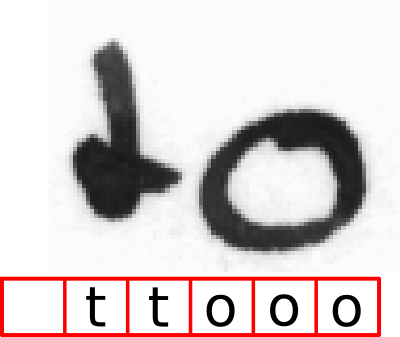
\includegraphics[width=0.6\textwidth]{img/Chap3/Annotation-image-CTC}
	\caption{ Annotation for each horizontal position of the image }
	\label{fig:Chap3-Annottion-image-CTC}
\end{figure}

CTC can solve both problems for us:
\begin{itemize}
	\item We can ignore both the position and width of the character in the image and only requires the text that occurs in the picture.
	\item Using decode techniques, we can directly get the result of the network, and no further post-processing of the recognized text is needed.
\end{itemize}

\subsection{Beam Search with CTC decoder}
CTC has more than the Decoding phase, it can have the Encoding, Loss calculation, but we don't need it in the thesis scope anymore. So, here, we only mention to CTC decoder, but in the way, it combines with Beam Search\cite{scheidl2018word}. Because CTC in decoding context can connect with another algorithm like best-path decoding, ...

\subsubsection{Beam search}

In computer science, beam search\cite{BeamSearch} is a heuristic search algorithm that explores a graph by expanding the most promising node in a limited set. Beam search is an optimization of best-first search the reduces its memory requirements. Best-first search is a graph search that orders all partial solutions (states) according to some heuristic. But in beam search, only a predetermined number of the best partial solutions are kept as candidates. Pseudocode for the basic version of beam-search is shown in Figure \ref{fig:Chap3-Basic-Version-BeamSearch}

\begin{figure}[H]
	\centering
	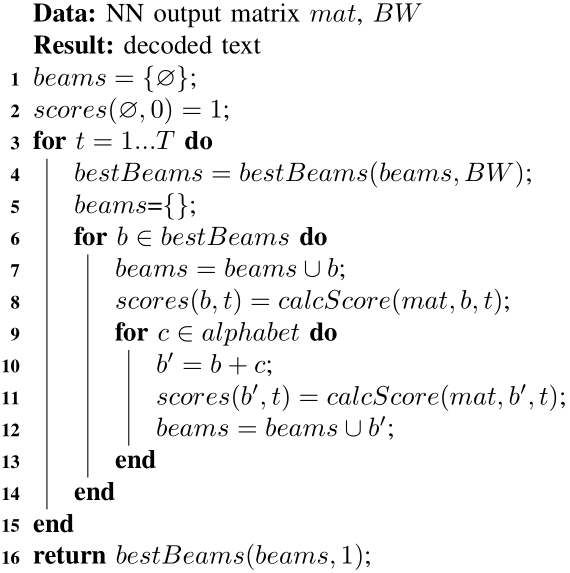
\includegraphics[width=0.8\textwidth]{img/Chap3/Basic-Version-BeamSearch}
	\caption{ Basic version of Beam Search }
	\label{fig:Chap3-Basic-Version-BeamSearch}
\end{figure}

% FIXME: Insert image about pseudo-code for beam-search

The beam search algorithm will be implemented through the following steps, with two parameters will be included: output matrix and beam width (BW), which specifies the number of beams to keep. First, the beam list and corresponding score are initialized (lines 1 and 2). After that, from 3-15, the algorithm will loop over all time-steps of the matrix output. At this point, only the best scoring beams (equal BW) from the previous time-step are kept (line 4). For each beam, we calculate the score and get a result (line 8); we will cover this step in more details later. Further, each beam is extended by all possible characters from the alphabet (line 10), and again, a score is calculated (line 11). After the last time-step, the best beams are returned (line 16).

% FIXME: Insert image about beam search

\begin{figure}[H]
	\centering
	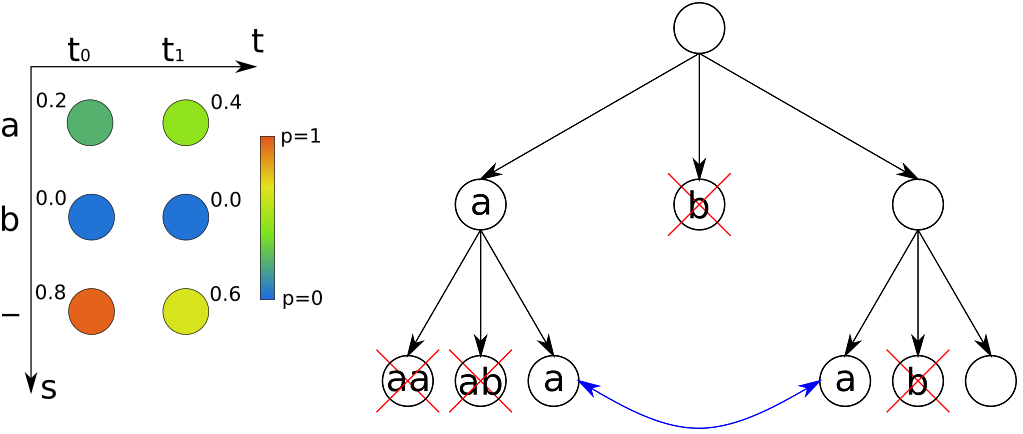
\includegraphics[width=\textwidth]{img/Chap3/BeamSearchTree}
	\caption{ NN output and tree of beams with alphabet = {"a", "b"} and BW = 2 }
	\label{fig:Chap3-BSTree}
\end{figure}

As we can see, in Figure \ref{fig:Chap3-BSTree}, the output matrices are decoded, and the tree of beams is shown. Beam search algorithm extended as possible and keep exactly BW candidates. Finally, we finished the last iteration, and the final step of the algorithm is to return the beam with the highest score, which is "a" in this example.

\subsubsection{Calculating the score}

As discussed above, in this part, we will talk about how to score the beam. We will split the beam-score into the score of paths ending with a blank(e.g. 'aa-') and paths ending with non-blank (e.g. 'aaa').

\begin{itemize}
	\item We denote the probability of all paths ending with a blank and corresponding to a beam b at time-step t
	      by $ P_{b}(b,t) $ and by $ P_{nb}(b,t) $ for the non-blank case.
	\item The probability $P_{tot}(b,t)$ of a beam b at time-step t is simply the sum of $P_b$ and $P_{nb}$, for example:
	      $P_{tot}(b,t) = P_b(b,t) + P_{nb}(b,t)$
\end{itemize}

\begin{figure}[H]
	\centering
	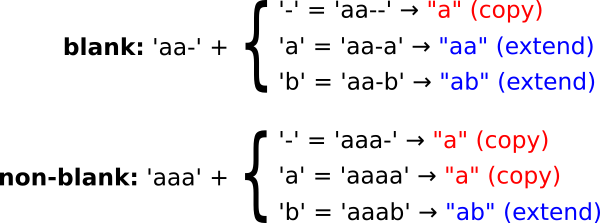
\includegraphics[width=0.7\textwidth]{img/Chap3/CTC_Scoring}
	\caption{ The effect of appending a character to paths ending with blank and non-blank }
	\label{fig:Chap3-CTC_Scoring}
\end{figure}

In Figure \ref{fig:Chap3-CTC_Scoring}, we will see what happens when we extend a path. Three main cases we can mention
is:
\begin{itemize}
	\item Extended by blank ('a' + '-' = 'a-')
	\item Extended by repeating last character ( 'aa' + 'a' = 'aaa' or 'aa-' + 'a' = 'aa-a')
	\item Extended by some other character ('aa' + 'b' = 'aab')
\end{itemize}

% FIXME: Viết lại các công thức bên dưới
And when we collapse the extended paths, two results we will get and some cases we needed to handle:
\begin{itemize}
	\item The unchanged (copied) beam ('a' $ \rightarrow $ 'a'):
	      \begin{itemize}
		      \item To copy a beam, we can extend corresponding paths by a blank and get
		            paths ending with a blank: $ P_b (n, t) += P_{tot}(b, t-1)*mat(blank, t) $
		      \item Besides, with the non-blank ending paths case, if we extend it by the last
		            character (the beam is not empty): $ P_{nb}(b,t) += P_{nb}(b,t-1)*mat(b[-1],t) $
		            with -1 indexes the last character in the beam
	      \end{itemize}
	\item An extended beam ('a' $\rightarrow$ 'aa' or 'ab'):
	      \begin{itemize}
		      \item To extend a beam. With the last character is different from the character we need
		            to extend, then there is no need for separating blanks ('-') in the paths:
		            $ P_{nb}(b+c,t) += P_{tot}(b,t-1)*mat(c,t) $
		      \item Or the last character of beam is repeated, we must ensure that the paths
		            end with a blank: $ P_{nb}(b+c,t) += P_b(b,t-1)*mat(c,t) $
		      \item We don't need to care about $P_b(b+c,t)$ because we added a non-blank character
	      \end{itemize}
\end{itemize}

\subsubsection{Putting it all together}

The CTC beam search algorithm is depicted in the Figure \ref{fig:Chap3-BS_CTC}. It is similar to the basic version that was previously shown. It does, however, contain the code for scoring the beams: copied beams (lines 7-10) and extended beams (lines 15-19). Finally, in order to find the best scoring beams, the program rates them using the Ptot (line 4) and then selects the best beams (BW).

\begin{figure}[H]
	\centering
	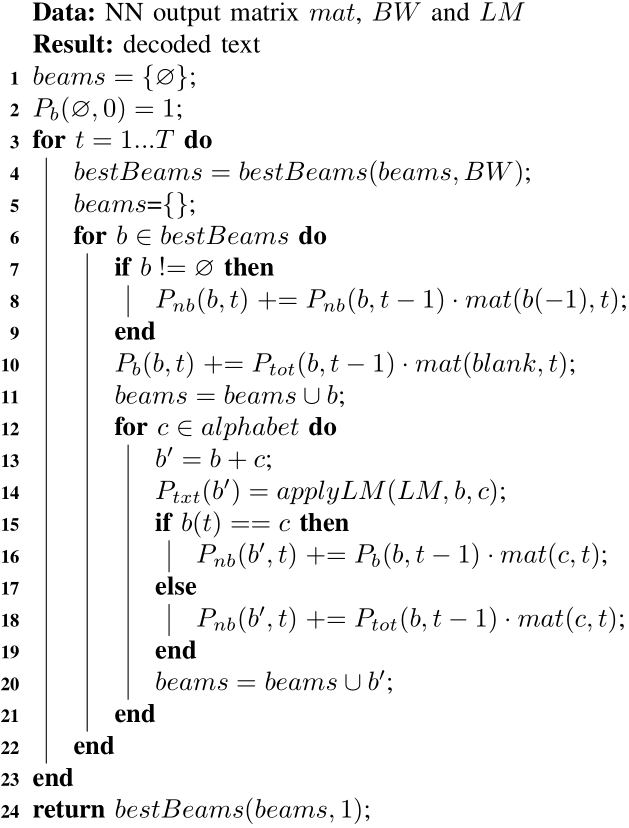
\includegraphics[width=0.8\textwidth]{img/Chap3/BS_CTC}
	\caption{ CTC beam search }
	\label{fig:Chap3-BS_CTC}
\end{figure}

\newpage
\section{Technology}
%FIX-ME: Chém gió thêm ra phần này, sử dụng ngôn ngữ gì bla bla 
% Ứng dụng được viết bằng react-native. Sử dụng hệ thống authenticate của firebase
Overall, the product app has been developed with technologies such as Java for Android apps and Firebase system authentication. Furthermore, to keep the application as light as possible, we use only native components and no external UI libraries.

% \subsection{React Native}

% \begin{figure}[H]
% 	\centering
% 	
\includegraphics[width=0.7\textwidth]{img/technology/ReactNative.png}
% 	\caption{React Native Logo}
% 	\label{fig:ReactNativeLogo}
% \end{figure}

% Traditional mobile app development necessitates knowledge of two distinct platforms (and programming languages): Android and iOS. However, using React Native\cite{ReactNative}, developers can create hybrid apps that operate on both platforms. The advantages of applying React Native in the app development process contain the following points.

% \begin{itemize}
% 	\item \textbf{Cross-Platform:} One of the significant advantages of React Native is that we can write the same code for both the Android and iOS ecosystems simultaneously, with just minor changes for each platform.
% 	\item \textbf{One programming language:} There is no need to be familiar with the languages used for platform-specific application development because React Native employs JavaScript, which is currently one of the most popular programming languages\cite{10MostPopularProgrammingLang}. To be more specific, in this project, we use an advanced version of JavaScript, which is known as TypeScript\cite{TypeScript}, and we will discuss it in the later Section.
% 	\item \textbf{Performance:} Because both platforms use the same code, React Native allows for the rapid creation of mobile applications. It also has a hot reloading functionality that ensures that modest changes to the program are shown to the developer right away.
% \end{itemize}

% Therefore, using this React Native framework benefits us in developing the same app for iOS devices from Apple Inc. According to the plan that we came up with before, when the product app works acceptably on Android devices, we will expand it and make it work on those iOS devices without massive effort when translating an app from one operating system to another.

% \subsection{TypeScript}

% \begin{figure}[H]
% 	\centering
% 	
\includegraphics[width=0.2\textwidth]{img/technology/JavaScript.png}
% 	\caption{JavaScript Logo}
% 	\label{fig:JavaScriptLogo}
% \end{figure}

% To know about TypeScript, first, we need to know JavaScript. JavaScript is a solid client-side programming language that is open-source. Its primary purpose is to enhance users' interaction with a web page. In other words, developers may make the website more dynamic and exciting by using this programming language. JavaScript is also widely used in the development of games and mobile apps. Excellent speed, cross-browser interoperability, and simple semantics are some of JavaScript's primary qualities, enabling a seamless development experience.

% \begin{figure}[H]
% 	\centering
% 	
\includegraphics[width=0.7\textwidth]{img/technology/TypeScript.png}
% 	\caption{TypeScript Logo}
% 	\label{fig:TypeScriptLogo}
% \end{figure}

% On the other hand, TypeScript is a modern JavaScript programming language. It is a statically built language for writing concise JavaScript code. It can be used with Node.js or any browser that supports ECMAScript 3 or above. Static typing, classes, and an interface are all available in TypeScript. Adopting Typescript for a large JavaScript project can result in more robust software easily deployable with a typical JavaScript application.

% \begin{itemize}
% 	\item \textbf{Static typing:} JavaScript is tightly typed, so it does not know what kind of variable it is dealing with until it is practically created at runtime. JavaScript now has type support thanks to TypeScript.
% 	\item \textbf{Supports new ECMAScript:} TypeScript may trans-pile unique ECMAScript criteria to ECMAScript objectives of our choice. As a result, we can use lambda, modules, functions, the spread operator, de-structuring, and classes, which are all features of ES2015 and beyond.
% 	\item \textbf{Type inference:} The use of type inference in TypeScript makes typing more manageable and less confusing. Even if we do not use the interface, TypeScript can help us avoid mistakes that could cause runtime issues.
% 	\item \textbf{Interoperability:} TypeScript is inextricably linked to JavaScript. As a result, it has high interoperability capabilities; however, it requires some additional work to integrate with TypeScript JS libraries.
% 	\item \textbf{Null examination strict:} In JavaScript software programming, errors, like cannot read property 'x' of undefined, are common. We may avoid most of these mistakes because a variable unknown to the TypeScript compiler cannot be used.
% \end{itemize}

% \subsection{NativeBase}

% \begin{figure}[H]
% 	\centering
% 	
\includegraphics[width=0.7\textwidth]{img/technology/nativebase-logo.png}
% 	\caption{NativeBase Logo}
% 	\label{fig:NativeBaseLogo}
% \end{figure}

% NativeBase\cite{NativeBase} is a component library for developers that want to create universal design systems. It is based on React Native and lets developers create apps for Android, iOS, and the web.

% \begin{itemize}
% 	\item \textbf{Highly themeable:} NativeBase's themeability is one of its most essential features. Make the app's theme and component styles as unique as we like, which means we can change the theme effortlessly.
%  \item \textbf{Rich component library:} As GeekyAnts stated, NativeBase has approximately 40 components to let developers create an app quickly and easily. It includes action sheets, menus, spinners, popovers, breadcrumbs, and valuable components.
%  \item \textbf{Out of the box accessibility:} By default, we can use all the provided components without changing them much. Moreover, the things they provide are designed with a high contrast ratio, making it more comfortable for the users when using the app.
% \end{itemize}

\subsection{Java}

\begin{figure}[H]
	\centering
	\includegraphics[width=0.7\textwidth]{img/technology/java.png}
	\caption{Java logo}
	\label{fig:JavaLogo}
\end{figure}

James Gosling developed Java at Sun Microsystems, Inc. in 1995, later acquired by Oracle Corporation. It's a straightforward programming language. Java makes programming easy to write, compile, and debug. It aids in the development of reusable code and modular programs.

Java is an object-oriented programming language based on classes that are designed to have as few implementation dependencies as feasible. Furthermore, Java is a general-purpose programming language that allows developers to write code once and run it on any device that supports Java. Java programs are compiled into byte code that may be run on any Java Virtual Machine. Besides, Java has a syntax that is similar to C and C++.

\subsection{Firebase}

\begin{figure}[H]
	\centering
	
\includegraphics[width=0.7\textwidth]{img/technology/firebase.png}
	\caption{FireBase logo}
	\label{fig:FireBaseLogo}
\end{figure}

Firebase is a web and mobile app development platform with simple and powerful APIs that don't require a server or backend. Firebase is a cloud-based platform. Also present is Google's server system. Its main goal is to make database operations simpler for users so they can program apps more easily. The real-time database service allows users to store and synchronize data. This is a completely cloud-based service. If the device is offline, it will use up its memory before automatically syncing with the server once it is online.

This feature largely comprises of backend services that help developers construct and manage their apps more effectively. The following services are included in this feature:

\begin{itemize}
	\item \textbf{Realtime database:} The Firebase Realtime Database is a cloud-based NoSQL database that processes data at millisecond speed. In the simplest sense, it can be thought of as a large JSON file.
 \item \textbf{Cloud firestore:} The Cloud Firestore is a NoSQL document database that allows users to store, sync, and query data from anywhere in the world using the app. It stores information in the form of documents, which are objects. It stores any data type, including text, binary data, and even JSON trees, using a key-value pair.
 \item \textbf{Authentication:} Using UI libraries and SDKs, the Firebase Authentication service makes it simple to authenticate users in the app. It reduces the time and effort required to develop and maintain the user authentication service. It even handles processes like account mergers, which can take a long time if done manually.
 \item \textbf{Remote configuration:} The remote configuration service speeds up the distribution of updates to users. Changes could range from updating UI components to altering application functionality. These are frequently used to deliver limited-time offers and content to a mobile application.
 \item \textbf{Hosting:} Firebase provides fast and secure application hosting. It can host both static and dynamic websites, as well as microservices. With a single command, it can host an application.
\end{itemize}
